\PassOptionsToPackage{unicode=true}{hyperref} % options for packages loaded elsewhere
\PassOptionsToPackage{hyphens}{url}
%
\documentclass[british,,jou,floatsintext]{apa6}
\usepackage{lmodern}
\usepackage{amssymb,amsmath}
\usepackage{ifxetex,ifluatex}
\usepackage{fixltx2e} % provides \textsubscript
\ifnum 0\ifxetex 1\fi\ifluatex 1\fi=0 % if pdftex
  \usepackage[T1]{fontenc}
  \usepackage[utf8]{inputenc}
  \usepackage{textcomp} % provides euro and other symbols
\else % if luatex or xelatex
  \usepackage{unicode-math}
  \defaultfontfeatures{Ligatures=TeX,Scale=MatchLowercase}
\fi
% use upquote if available, for straight quotes in verbatim environments
\IfFileExists{upquote.sty}{\usepackage{upquote}}{}
% use microtype if available
\IfFileExists{microtype.sty}{%
\usepackage[]{microtype}
\UseMicrotypeSet[protrusion]{basicmath} % disable protrusion for tt fonts
}{}
\IfFileExists{parskip.sty}{%
\usepackage{parskip}
}{% else
\setlength{\parindent}{0pt}
\setlength{\parskip}{6pt plus 2pt minus 1pt}
}
\usepackage{hyperref}
\hypersetup{
            pdftitle={An excess of positive results: Comparing the standard Psychology literature with Registered Reports},
            pdfkeywords={Publication bias, Registered Reports, hypothesis testing},
            pdfborder={0 0 0},
            breaklinks=true}
\urlstyle{same}  % don't use monospace font for urls
\usepackage{graphicx,grffile}
\makeatletter
\def\maxwidth{\ifdim\Gin@nat@width>\linewidth\linewidth\else\Gin@nat@width\fi}
\def\maxheight{\ifdim\Gin@nat@height>\textheight\textheight\else\Gin@nat@height\fi}
\makeatother
% Scale images if necessary, so that they will not overflow the page
% margins by default, and it is still possible to overwrite the defaults
% using explicit options in \includegraphics[width, height, ...]{}
\setkeys{Gin}{width=\maxwidth,height=\maxheight,keepaspectratio}
\setlength{\emergencystretch}{3em}  % prevent overfull lines
\providecommand{\tightlist}{%
  \setlength{\itemsep}{0pt}\setlength{\parskip}{0pt}}
\setcounter{secnumdepth}{0}
% Redefines (sub)paragraphs to behave more like sections
\ifx\paragraph\undefined\else
\let\oldparagraph\paragraph
\renewcommand{\paragraph}[1]{\oldparagraph{#1}\mbox{}}
\fi
\ifx\subparagraph\undefined\else
\let\oldsubparagraph\subparagraph
\renewcommand{\subparagraph}[1]{\oldsubparagraph{#1}\mbox{}}
\fi

% set default figure placement to htbp
\makeatletter
\def\fps@figure{htbp}
\makeatother

\usepackage{etoolbox}
\makeatletter
\providecommand{\subtitle}[1]{% add subtitle to \maketitle
  \apptocmd{\@title}{\par {\large #1 \par}}{}{}
}
\makeatother
% Manuscript styling
\usepackage{csquotes}
\usepackage{upgreek}
\captionsetup{font=singlespacing,justification=justified}

% Table formatting
\usepackage{longtable}
\usepackage{lscape}
% \usepackage[counterclockwise]{rotating}   % Landscape page setup for large tables
\usepackage{multirow}		% Table styling
\usepackage{tabularx}		% Control Column width
\usepackage[flushleft]{threeparttable}	% Allows for three part tables with a specified notes section
\usepackage{threeparttablex}            % Lets threeparttable work with longtable

% Create new environments so endfloat can handle them
% \newenvironment{ltable}
%   {\begin{landscape}\begin{center}\begin{threeparttable}}
%   {\end{threeparttable}\end{center}\end{landscape}}
\newenvironment{lltable}{\begin{landscape}\begin{center}\begin{ThreePartTable}}{\end{ThreePartTable}\end{center}\end{landscape}}

% Enables adjusting longtable caption width to table width
% Solution found at http://golatex.de/longtable-mit-caption-so-breit-wie-die-tabelle-t15767.html
\makeatletter
\newcommand\LastLTentrywidth{1em}
\newlength\longtablewidth
\setlength{\longtablewidth}{1in}
\newcommand{\getlongtablewidth}{\begingroup \ifcsname LT@\roman{LT@tables}\endcsname \global\longtablewidth=0pt \renewcommand{\LT@entry}[2]{\global\advance\longtablewidth by ##2\relax\gdef\LastLTentrywidth{##2}}\@nameuse{LT@\roman{LT@tables}} \fi \endgroup}

% \setlength{\parindent}{0.5in}
% \setlength{\parskip}{0pt plus 0pt minus 0pt}

% Overwrite redefinition of paragraph and subparagraph by the default LaTeX template
% See https://github.com/crsh/papaja/issues/292
\makeatletter
\renewcommand{\paragraph}{\@startsection{paragraph}{4}{\parindent}%
  {0\baselineskip \@plus 0.2ex \@minus 0.2ex}%
  {-1em}%
  {\normalfont\normalsize\bfseries\itshape\typesectitle}}

\renewcommand{\subparagraph}[1]{\@startsection{subparagraph}{5}{1em}%
  {0\baselineskip \@plus 0.2ex \@minus 0.2ex}%
  {-\z@\relax}%
  {\normalfont\normalsize\itshape\hspace{\parindent}{#1}\textit{\addperi}}{\relax}}
\makeatother

% \usepackage{etoolbox}
\makeatletter
\patchcmd{\HyOrg@maketitle}
  {\section{\normalfont\normalsize\abstractname}}
  {\section*{\normalfont\normalsize\abstractname}}
  {}{\typeout{Failed to patch abstract.}}
\makeatother
\shorttitle{Positive Results in Standard vs Registered Reports}
\author{Anne M. Scheel\textsuperscript{1}, Mitchell Schijen\textsuperscript{1}, \& Daniël Lakens\textsuperscript{1}}
\affiliation{
\vspace{0.5cm}
\textsuperscript{1} Eindhoven University of Technology}
\authornote{

Correspondence concerning this article should be addressed to Anne M. Scheel, Den Dolech 1, Atlas 9.417, 5600 MB, Eindhoven, The Netherlands. E-mail: a.m.scheel@tue.nl}
\keywords{Publication bias, Registered Reports, hypothesis testing}
\usepackage{dblfloatfix}


\usepackage{float}
\usepackage{framed}
\usepackage{caption}
\usepackage{setspace}
\captionsetup[figure]{font={stretch=1, small}, skip=10pt}
\captionsetup[textbox]{name=Box,labelsep=period,labelfont=it}
\newfloat{textbox}{thp}{lop}
\floatname{textbox}{Box}
\ifnum 0\ifxetex 1\fi\ifluatex 1\fi=0 % if pdftex
  \usepackage[shorthands=off,main=british]{babel}
\else
  % load polyglossia as late as possible as it *could* call bidi if RTL lang (e.g. Hebrew or Arabic)
  \usepackage{polyglossia}
  \setmainlanguage[variant=british]{english}
\fi

\title{An excess of positive results: Comparing the standard Psychology literature with Registered Reports}

\date{}

\abstract{
When studies with positive results that support the tested hypotheses have a higher probability of being published than studies with negative results, the literature will give a distorted view of the evidence for scientific claims. Psychological scientists have been concerned about the degree of distortion in their literature due to publication bias and inflated Type-1 error rates. Registered Reports were developed with the goal to minimise such biases: In this new publication format, peer review and the decision to publish take place before the study results are known. We compared the results in the full population of published Registered Reports in Psychology (\(N = 71\) as of November 2018) with a random sample of hypothesis-testing studies from the standard literature (\(N = 152\)) by searching 633 journals for the phrase `test* the hypothes*' (replicating a method by Fanelli, 2010). Analysing the first hypothesis reported in each paper, we found \(96\%\) positive results in standard reports, but only \(44\%\) positive results in Registered Reports. The difference remained nearly as large when direct replications were excluded from the analysis (\(96\%\) vs \(50\%\) positive results). This large gap suggests that psychologists under-report negative results to an extent that threatens cumulative science. Although our study did not directly test the effectiveness of Registered Reports at reducing bias, these results show that the introduction of Registered Reports has led to a much larger proportion of negative results appearing in the published literature compared to standard reports.
}

\begin{document}
\maketitle

If the scientific literature were a faithful representation of the research scientists conduct, a cumulative science would be a powerful tool to infer what is true about the world.
When random error is the only threat to the accuracy of individual findings, aggregating across many findings allows inferences about the presence and size of effects with a certain reliability.
But when published findings are systematically biased, cumulative science breaks down:
Unlike random error, bias does not cancel out when aggregating across studies -- in the worst case it accumulates, leading us away from the truth rather than towards it.
Unfortunately there are good reasons to believe that the Psychology literature is not a faithful representation of all research psychologists conduct.
For more than half a century, scientists have repeatedly noticed a suspiciously high \enquote{success} rate in Psychology:
Studying 362 empirical articles published in four Psychology journals in 1955/56, Sterling (1959) found that \(97.28\%\) of the studies that used significance tests rejected the null hypothesis.
A replication of this study performed on articles published in 1986/87 reported \(95.56\%\) statistically significant results (Sterling, Rosenbaum, \& Weinkam, 1995).
Similarly, a seminal study by Fanelli (2010) compared the literatures of 20 disciplines and found that \(91.5\%\) of papers published in Psychology reported support for their first hypothesis, the highest estimate of all disciplines in the study.
For these percentages to be a realistic representation of the research that psychologists perform, both statistical power and the proportion of true hypotheses (i.e., the prior probability that the null hypothesis is false) that are tested must exceed \(90\%\).
In other words: nearly all predictions researchers make must be correct, and either the studied effect sizes or the used sample sizes (given the same study design) must consistently be very large.

\hypertarget{a-biased-literature}{%
\subsection{A biased literature}\label{a-biased-literature}}

Sterling (1959) already suspected a selection process behind the numbers he found:
\enquote{(\ldots{}) for psychological journals a policy exists under which the vast majority of published articles satisfy a minimum criterion of {[}statistical{]} significance} (p.~31).
This selection process is one of several kinds of biases that will lead to an inflation of positive results in the literature.
We can distinguish two broad categories of bias: \enquote{publication bias} and \enquote{questionable research practices}.
Publication bias describes publishing behaviours that give manuscripts that find support for their tested hypotheses a higher chance of being published than manuscripts that do not find support for their tested hypotheses.
These include editors and reviewers selectively rejecting manuscripts with negative results (``reviewer bias'', Greenwald, 1975; Mahoney, 1977) and researchers deciding not to submit studies with negative results for publication (``file-drawering''; Rosenthal, 1979).
Questionable research practices (QRPs) describe research behaviours that make the evidence in favour of a certain conclusion look stronger than it is (typically, though not always, leading to an inflated type-I error rate; see Lakens, 2019).
These include presenting unexpected results as having been predicted \emph{a priori} (HARKing, short for ``hypothesising after results are known''; Kerr, 1998) and exploiting flexibility in data analysis to obtain statistically significant results (``\emph{p}-hacking''; Simmons, Nelson, \& Simonsohn, 2011).
Evidence for both categories of bias exist:
Publication bias has been shown in peer review (Atkinson, Furlong, \& Wampold, 1982; Mahoney, 1977) and in longitudinal data from an NSF grant programme that found a file-drawering effect for studies with negative results (Franco, Malhotra, \& Simonovits, 2014, 2016); and QRPs have been admitted by scientists in several survey studies (Agnoli, Wicherts, Veldkamp, Albiero, \& Cubelli, 2017; Fiedler \& Schwarz, 2016; John, Loewenstein, \& Prelec, 2012).

Some have argued that selecting for statistically significant results is defensible -- desirable, even -- because it weeds out low-quality research that would only pollute the literature (Cleophas \& Cleophas, 1999; see also de Winter \& Happee, 2013; and van Assen, van Aert, Nuijten, \& Wicherts, 2014, for a critique).
How problematic selective publishing is in practice remains an empirical question:
If most negative results that are currently missing from the literature are the result of immature ideas or poorly conducted studies, we should expect that a literature in which studies are selected based on their quality but not based on their results would contain a similar proportion of positive results as the current one.
But how many positive results would such an unbiased literature contain in reality?
We set out to explore this question by comparing the rate of positive results in the current Psychology literature to studies published in a new format designed to minimise QRPs and publication bias: Registered Reports.

\hypertarget{methods-to-mitigate-bias}{%
\subsection{Methods to mitigate bias}\label{methods-to-mitigate-bias}}

An increasingly popular proposal to reduce bias is preregistration, where authors register a time-stamped protocol of their hypotheses, planned method, and analysis plan before data collection (for a historical overview, see Wiseman, Watt, \& Kornbrot, 2019).
Preregistration is thought to mitigate QRPs by preventing HARKing (hypotheses must be stated before the results are known) and by reducing the risk of \emph{p}-hacking via restricted flexibility in data analysis.
However, preregistration does not prevent file-drawering or reviewer bias and may thus be insufficient to fight publication bias (Goldacre et al., 2016; Rasmussen, Lee, \& Bero, 2009; but see Kaplan \& Irvin, 2015).
A more effective safeguard against both publication bias and QRPs is promised by Registered Reports (Chambers, 2013; Chambers, Dienes, McIntosh, Rotshtein, \& Willmes, 2015; Jonas \& Cesario, 2016; Nosek \& Lakens, 2014).
Registered Reports (RRs) are a new publication format with a restructured submission timeline:
Before collecting data, authors submit a study protocol containing their hypotheses, planned procedures, and analysis pipeline (typically in the form of an Introduction and Method section) to a journal.
The protocol undergoes peer review, and, if successful, receives \enquote{in-principle acceptance}, meaning that the journal commits to publishing the final article following data collection, regardless of the statistical significance of the results.
The authors then collect and analyse the data and complete the final report.
The final report undergoes another round of peer review, but this time only to ensure that the authors adhered to the registered plan and did not draw unjustified conclusions (and, if applicable, that the data pass pre-specified quality checks).
Registered Reports thus combine an antidote to QRPs (preregistration) with an antidote to publication bias, because studies are selected for publication before their results are known.
Since its introduction at the journal \emph{Cortex} in 2013, the format has rapidly gained popularity and is offered by 225 journals at the time of writing (\url{http://cos.io/rr}).

In addition to bias protection, Registered Reports promise high-quality research: Stage-1 (pre-data) peer review increases the likelihood that methodological flaws and immature or misguided ideas will be identified and addressed before a study is conducted, and authors typically have to include outcome-neutral control conditions that allow verifying data quality once results are in (studies failing these quality checks may be rejected).
Many journals offering Registered Reports also require that planned hypothesis tests are based on a power analysis that ensures a high probability of finding a statistically significant result if there is a true effect of the expected size (e.g., \(90\%\) power for a given effect size of interest\footnote{An overview of the requirements specified by each participating journal is available at \url{https://docs.google.com/spreadsheets/d/1D4_k-8C_UENTRtbPzXfhjEyu3BfLxdOsn9j-otrO870}}).

Assuming a constant alpha level, the rate of positive results in a literature (i.e., the proportion of supported hypotheses among all tested hypotheses) is influenced by three factors: the proportion of true hypotheses among all tested hypotheses, statistical power, and bias.
The Registered Reports format combines powerful safeguards against publication bias and QRPs with standards for research quality that are at least equal to ordinary peer review, and often include statistical power requirements that likely exceed those in the standard literature (see e.g., Maxwell, 2004; Singleton Thorn, Dudgeon, \& Fidler, 2019; Szucs \& Ioannidis, 2017).
Therefore, if the emerging Registered Reports literature in Psychology contains fewer positive results than the standard literature, the cause must be either the difference in bias or a lower proportion of true hypotheses tested in Registered Reports (or a combination of the two).
At this time, we have good reasons to believe in a difference in bias, but less reason to believe in a difference in the proportion of true hypotheses (at least regarding original work, see below), which would make bias a more plausible explanation of a potential difference in the positive result rate.
Considering the high standards for research quality in Registered Reports, a large difference in positive results between Registered Reports and the standard literature would also indicate that publication bias is not a desirable filter for poorly conducted studies, but that we should worry about high-quality negative results we are missing because of it.

\hypertarget{the-current-study}{%
\subsection{The current study}\label{the-current-study}}

The goal of our study was to test if Registered Reports in Psychology show a lower positive result rate than articles published in the traditional way (henceforth referred to as \enquote{standard reports}, SRs), and to estimate the size of this potential difference.
We set out to replicate a study by Fanelli (2010) on a new sample of standard reports in Psychology and compared them to all published Registered Reports in Psychology.
Fanelli searched for articles containing the phrase \enquote{test\(^\ast\) the hypothes\(^\ast\)}, drew a random sample of 150 articles per discipline, and for each of these coded if the first hypothesis mentioned in the abstract or full text had been supported or not.
For standard reports we used the same sampling method (restricted to the Psychology discipline), and for Registered Reports we relied on a database curated by the Center for Open Science (COS).
We chose this method because Fanelli's 2010 and 2012 studies (both use the same coding method) have been highly influential, and his method can easily be applied to a large set of studies.
We additionally coded if studies were replications or original work because many published Registered Reports are replications.
If replications are motivated by scepticism of the original results, the prior probability of hypotheses tested in these studies may be lower than in original studies, which could lead to a larger proportion of negative results regardless of bias.

In a recent commentary on benefits and challenges of open-science practices for early-career researchers, Allen and Mehler (2019) conducted a similar investigation:
They coded the proportion of null results in the 127 biomedical and Psychology Registered Reports listed in the COS database as of September 2018.
We were not aware of their parallel efforts when we planned our study in September and October 2018.
Allen and Mehler used a self-developed method to code the percentage of unsupported hypotheses in Registered Reports (counting all hypotheses in each paper) and found \(60.5\%\) unsupported hypotheses across all included Registered Reports, \(66\%\) for replication attempts, and \(54.5\%\) for novel research.
They compared these numbers to an estimate of 5--20\(\%\) null results in the standard literature (based on data from Fanelli, 2012, who coded only the first hypothesis of each paper; and Cristea \& Ioannidis, 2018, who coded the percentage of statistically significant results in figures and tables of articles published in Nature, Science, and PNAS).

A major advantage of our study is that it allows us to draw a more meaningful comparison between Registered Reports and the standard literature because we apply a previously used method (Fanelli, 2010, 2012) to both groups.
In addition, we replicate Fanelli (2010) and provide data to evaluate his method: The search term \enquote{test\(^\ast\) the hypothes\(^\ast\)} might introduce selection effects, meaning that results obtained this way may not generalise to hypothesis-testing studies that do not use this phrase.
Therefore we also coded the phrases used to introduce hypotheses in Registered Reports, analysed how many of them would have been detected with Fanelli's search term, and compiled a list of alternative search terms to test the generalisability of Fanelli's results in the future.
Finally, we share a rich dataset containing the exact quotes of hypotheses and conclusions on which we based our judgements, as well as detailed descriptions of our sampling and coding procedure (see Appendix).
This allows others to verify (or contest) our results and may provide an interesting resource for future meta-scientific research.

\hypertarget{methods}{%
\section{Methods}\label{methods}}

After conducting a pilot to test the planned procedure, we preregistered our study (\url{https://osf.io/s8e97}).
Methods and analyses described here were preregistered unless otherwise noted.
A detailed comparison of our preregistration and the eventual procedure is provided in the supplement.
We report how we determined our sample size, all data exclusions, and all measures in the study.

\hypertarget{sample}{%
\subsection{Sample}\label{sample}}

We used the same method as Fanelli (2010) to obtain a new sample of standard reports, but restricted year of publication to 2013-2018 to match the sample to the Registered Reports population.
We excluded papers if they were incomplete, unpublished, or retracted articles (e.g., meeting abstracts, study protocols without results), if they did not test a hypothesis, or if they contained insufficient information to reach a coding decision.
An overview of the sampling process and all exclusions is shown in Figure~\ref{fig:sampling}.

For standard reports we downloaded a current version of the Essential Science Indicators (ESI) database (retrieved on 4th December 2018) and used Web of Science to search for articles published between 2013 and 2018 with a Boolean search query containing the phrase \enquote{test\(^\ast\) the hypothes\(^\ast\)} and the ISSNs of all 633 journals listed in the ESI Psychiatry/Psychology category.
Using the same sample size as Fanelli (2010), we randomly selected 150 papers from the 1919 search results using the sample() function in R and the seed \enquote{20190120} (seed was not preregistered, but no other seeds were tried).
We initially excluded eight papers and replaced them (decision to replace excluded papers was not preregistered) through the same random sampling procedure until 150 studies were found that met our criteria, but later found that two papers had been excluded erroneously, leading to a final sample size of 152 (see Fig.~\ref{fig:sampling}).



\begin{figure*}
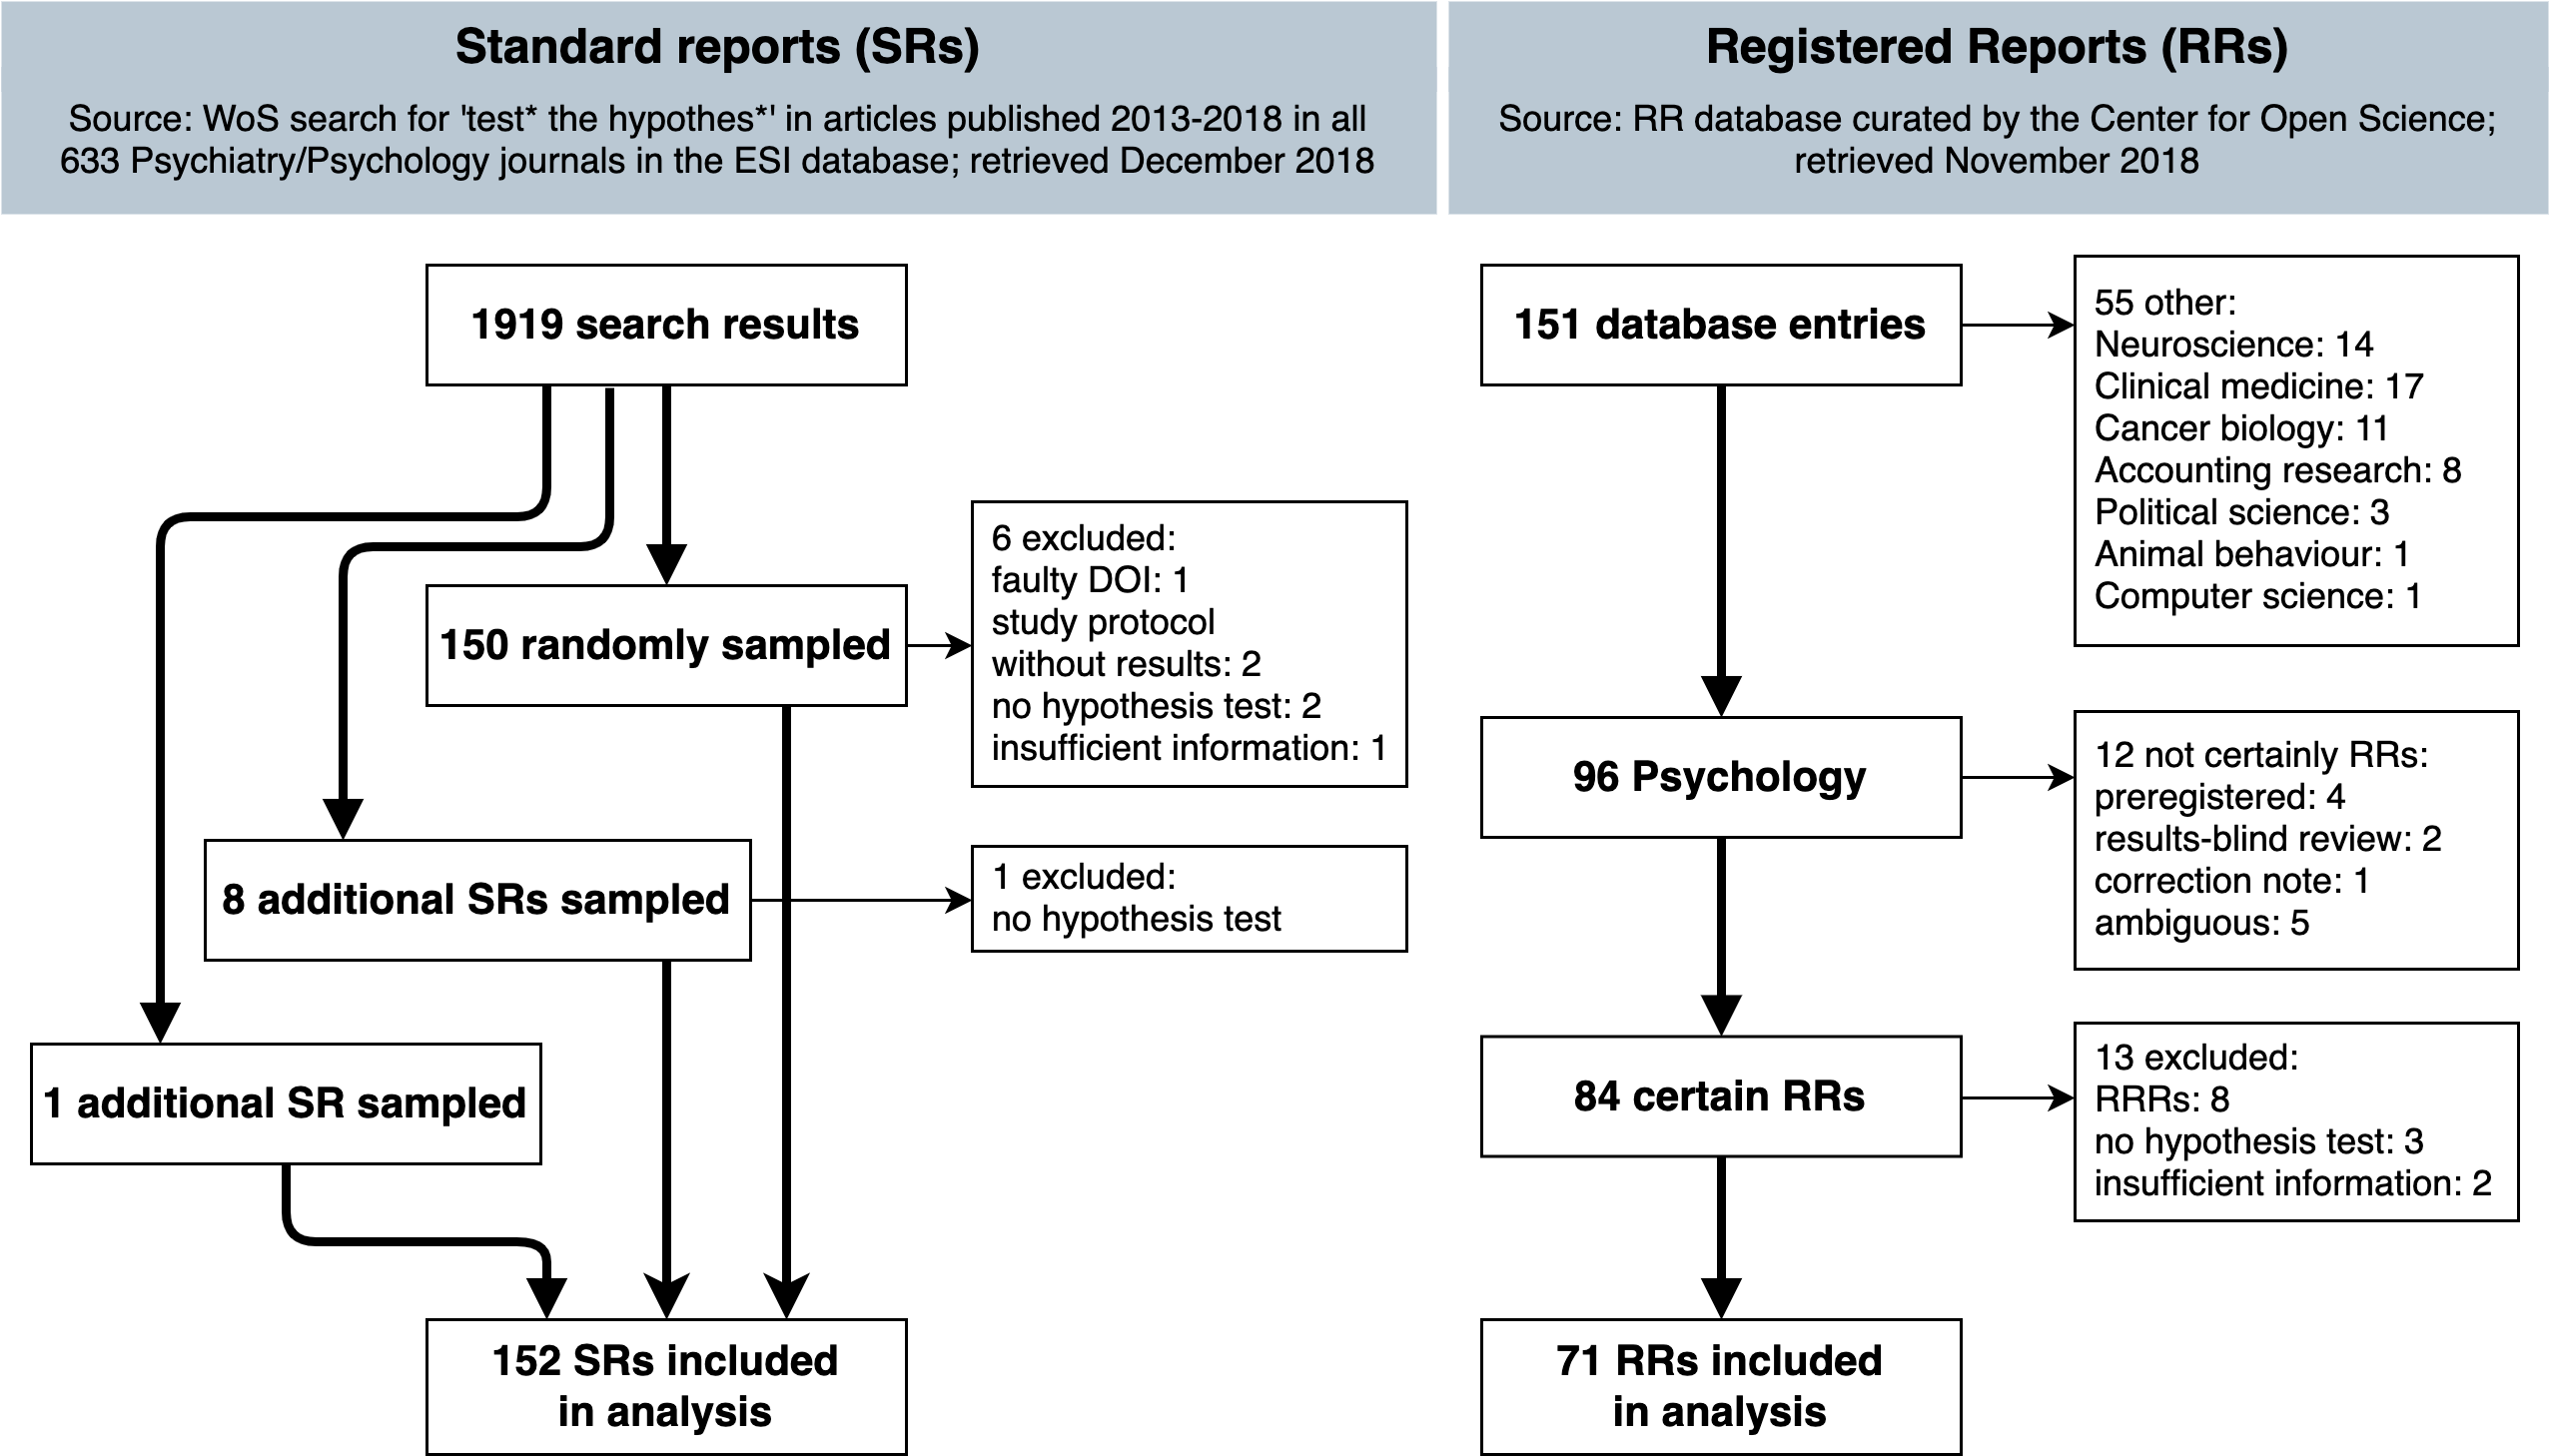
\includegraphics[width=\textwidth]{sampling_process_flowchart} \caption{Sampling process and exclusions for standard reports and Registered Reports. Standard reports were accidentally oversampled: We initially excluded 8 papers and only after replacing them found that two had been excluded erroneously. \enquote{Preregistered}: study had been preregistered but was not a full RR; \enquote{results-blind review}: article had undergone results-blind peer review but was not a full RR (authors knew results before first submission); \enquote{ambiguous}: four of these had been treated as Registered Reports but used pre-existing data to which the authors had access before conducting their analyses, one had no explicit signs of an RR except for a 2.5-year delay between submission and acceptance (we chose to exclude these cases to be conservative).}\label{fig:sampling}
\end{figure*}

For Registered Reports we aimed to include all published Registered Reports in the field of Psychology that tested at least one hypothesis, regardless of whether or not they used the phrase \enquote{test\(^\ast\) the hypothes\(^\ast\)}.
We downloaded a database of published Registered Reports curated by the Center for Open Science\footnote{\url{https://www.zotero.org/groups/479248/osf/items/collectionKey/KEJP68G9}} (retrieved on 19th November 2018), and excluded papers published in journals that were listed in categories other than \enquote{Psychiatry/Psychology} or \enquote{Multidisciplinary} in the ESI.
Note that the decision to focus only on the Psychiatry/Psychology category meant excluding 13 Registered Reports published in \emph{Cortex} because the ESI counts this journal towards the separate category \enquote{Neuroscience and Behavior}.
Papers published in multidisciplinary journals and in journals not included in the ESI (e.g., \emph{Royal Society Open Science}) were hand-coded by AS.
This deviates from our preregistration insofar as we had not specified how discipline membership would be determined.

Following these exclusions, we verified the Registered Reports status of all remaining papers in our sample.
Papers were counted as Registered Reports if they were labelled as such by the journal itself and the journal submission guidelines made it clear that these submissions had been reviewed and received in-principle acceptance before the data collection (or analyses) of all studies in the paper had been conducted (in accordance with \url{https://cos.io/rr}).
For papers not clearly labelled as Registered Reports, we consulted relevant editorial publications (e.g., for special issues) or contacted the respective editors directly.
Of the 151 entries in the COS Registered Reports database, 55 were excluded because they belonged to a non-Psychology discipline, 12 because we could not verify that they were Registered Reports, and 13 because they did not test hypotheses or contained insufficient information, leaving 71 Registered Reports for the final analysis (see Fig.~\ref{fig:sampling}).
Note that we excluded all eight \enquote{Registered Replication Reports} (RRRs; Simons, Holcombe, \& Spellman, 2014; Simons, 2018) in our sample because this format explicitly focusses on effect size estimation and not hypothesis testing (``Registered Replication Reports,'' n.d., decision was not preregistered).

\hypertarget{measures-and-coding-procedure}{%
\subsection{Measures and coding procedure}\label{measures-and-coding-procedure}}

The main dependent variable was whether the first hypothesis was supported or not, as reported by the authors.
We tried to follow Fanelli's (2010) coding procedure as closely as possible, which he describes as follows:

\begin{quote}
By examining the abstract and/or full- text, it was determined whether the authors of each paper had concluded to have found a positive (full or partial) or negative (null or negative) support.
If more than one hypothesis was being tested, only the first one to appear in the text was considered.
We excluded meeting abstracts and papers that either did not test a hypothesis or for which we lacked sufficient information to determine the outcome. (p.~8)
\end{quote}

Like Fanelli (2010), we coded hypotheses as having received \enquote{support}, \enquote{partial support}, or \enquote{no support}, which was recoded into a binary \enquote{support} (full or partial) vs \enquote{no support} variable for the analysis.
Coding disagreements between full and partial support were deemed minor since they would not affect the final results. Thus, only disagreements affecting the binary support/no support classification were treated as major and resolved through discussion.

Before preregistering our study, we conducted a pilot to assess if we could employ Fanelli's method successfully.
Originally we had planned to first reproduce his results on the same sample of Psychiatry/Psychology articles used in Fanelli (2010).
Unfortunately the author refused to share the original data (or even a list of the coded articles) with us.
Instead, we received an excerpt which contained data for 11 records from the original sample, but no reference information of the coded articles (personal communication, 5th October 2018).
We were able to find these 11 articles based on the hypothesis quotes that had been coded, and used them as a pilot sample along with 10 randomly selected Registered Reports.
MS and AS independently coded all 21 pilot articles with only one major disagreement in each group.
In the standard reports group, this disagreement was also the only case of major disagreement with Fanelli's original coding, which we deemed satisfying to proceed.

Based on our experiences during the pilot, we added one coding criterion:
If the first hypothesis mentioned in a paper was not explicitly tested but subsequently divided into sub-hypotheses that were tested, we would code the first \emph{tested} hypothesis rather than the first hypothesis mentioned in the text.
In Registered Reports we coded the first preregistered hypothesis, thus excluding unregistered pilot studies.
MS coded all papers in the sample, AS double-coded all papers MS had found difficult to code or could not code (\(24\) RRs and \(47\) SRs).
Only 3 disagreements were major (Cohen's kappa = .808) and subsequently resolved by discussion; 15 were minor (disagreement between \enquote{support} and \enquote{partial support}).
We had preregistered that AS would additionally code a random subset of both groups, but decided against it because the number of double-coded papers seemed sufficient after double-coding only the difficult cases.

\hypertarget{hypothesis-introductions}{%
\subsubsection{Hypothesis introductions}\label{hypothesis-introductions}}

Selecting papers that use the phrase \enquote{test\(^\ast\) the hypothes\(^\ast\)} might yield different results than alternative search phrases.
Getting a better overview of \enquote{natural} descriptions of hypotheses would be useful for future investigations of the generalisability of Fanelli's (2010) results and could inspire new research questions.
We therefore extracted the phrase used to introduce the hypothesis from the coded hypothesis quotes for all Registered Reports and tried to identify clusters of similar expressions which may be used to create alternative search phrases.

\hypertarget{replication-status}{%
\subsubsection{Replication status}\label{replication-status}}

We also wanted to code if a study was a replication of a previously published one:
We expected a much larger proportion of Registered Reports to be direct replications, many of which may have been motivated by scepticism of the original study.
A lower positive result rate in Registered Reports could then be an effect of failed replications rather than an effect of safeguards against QRPs and publication bias.
After an initial coding attempt with ill-defined coding criteria had led to too many disagreements (described further in the Appendix), we developed the following strategy (not pre-registered):
We searched the full texts of all papers for the string \enquote{replic\(^\ast\)} (cf. Makel, Plucker, \& Hegarty, 2012; Köhler \& Cortina, 2019; Mueller-Langer, Fecher, Harhoff, \& Wagner, 2019; Pridemore, Makel, \& Plucker, 2018) and, for papers that did contain it, determined whether the coded hypothesis was a close replication with the goal to verify a previously published result.
Conceptual replications and internal replications (replication of a study in the same paper) were not counted as replications in this narrow sense, since both are more likely to be motivated by the goal to build on previous work than by scepticism.
AS coded all papers, DL double-coded 32 Registered Reports (\(45.07 \%\)) and 99 standard reports (\(65.13 \%\)).
There were 5 disagreements (Cohen's kappa = .878), all were resolved by discussion.

\hypertarget{additional-measures}{%
\subsubsection{Additional measures}\label{additional-measures}}

All additional measures we collected but have not described thus far were either auxiliary variables to facilitate the coding process or earlier versions of the variables discussed above.
All of these are documented in the Appendix and in our shared dataset and codebook.

\hypertarget{analysis}{%
\subsection{Analysis}\label{analysis}}

We planned to test our hypothesis in the following way (quoting directly from our preregistration, \url{https://osf.io/sy927}):

\begin{quote}
A one-sided proportion test with an alpha level of \(5\%\) will be performed to test whether the positive result rate (full or partial support) of Registered Reports in psychology is statistically lower than the positive result rate of conventional reports\footnote{We later changed the term to \enquote{standard reports}.} in psychology.
In addition to testing if there is a statistically significant difference between RRs and conventional reports, we will test if the difference is smaller than our smallest effect size of interest using an equivalence test for proportion tests with an alpha level of \(5\%\) (Lakens, Scheel, \& Isager, 2018).
We determined our smallest effect size of interest to be the difference between the positive result rate in psychology (\(91.5\%\)) and the positive result rate in general social sciences (\(85.5\%\)) as reported by Fanelli (2010), i.e.~a difference of \(91.5\% - 85.5\% = 6\%\).
The rationale for choosing general social sciences as a comparison is that this discipline had the lowest positive result rate amongst the \enquote{soft} sciences (Fanelli, 2010).
The exact percentage for general social sciences was extracted from Figure 1 in Fanelli (2010) using the software WebPlotDigitizer (Rohatgi, 2018).
\end{quote}

We would accept our hypothesis that Registered Reports have a lower positive result rate than standard reports if we found a negative difference between Registered Reports and standard reports that was significantly different from 0 \emph{and} not statistically equivalent to a range from \(-6\%\) to \(+6\%\) (both at \(\alpha = 5\%\)).

\hypertarget{results}{%
\section{Results}\label{results}}

\hypertarget{confirmatory-analyses}{%
\subsection{Confirmatory Analyses}\label{confirmatory-analyses}}

146 out of 152 standard reports and 31 out of 71 Registered Reports had positive results, meaning that the positive result rate was \(96.05 \%\) for standard reports (\(95 \%\) CI {[}91.61, 98.54{]}) and \(43.66 \%\) for Registered Reports (\(95 \%\) CI {[}31.91, 55.95{]}; see Fig.~\ref{fig:mainplot}).
The preregistered one-sided proportions test with an alpha level of \(5\%\) showed that this difference of \(52.39 \%\) was statistically significant, \(\chi^2 = 77.96\), \(p < .001\).
Unsurprisingly, the difference was not statistically equivalent to a range between \(-6 \%\) and \(6 \%\) at \(\alpha = 5\%\), \(z = 7.61\), \(p > .999\), meaning that we cannot reject differences more extreme than \(6\%\).
We thus accept our hypothesis that the positive result rate in Registered Reports is lower than in standard reports.



\begin{figure}
\centering
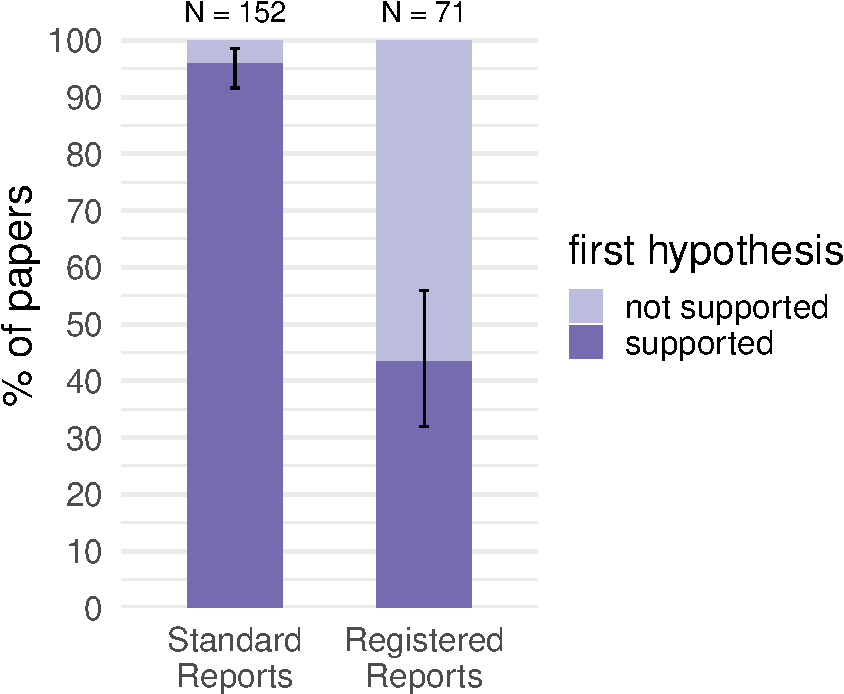
\includegraphics{positive_results_SRs_RRs_files/figure-latex/mainplot-1.pdf}
\caption{\label{fig:mainplot}Positive result rates for standard reports and Registered Reports. Error bars indicate \(95 \%\) confidence intervals around the observed positive result rate.}
\end{figure}

\hypertarget{exploratory-analyses}{%
\subsection{Exploratory Analyses}\label{exploratory-analyses}}

As described in the Method section, we only classified direct replications of previously published work as replications.
This means that our non-replication category also contains some conceptual replications and \enquote{internal} replications (where original and replication are published in the same paper).
For ease of communication we will nonetheless refer to this category as \enquote{original} studies.
As expected, direct replications were much more common among Registered Reports than standard reports: 41 out of 71 Registered Reports (\(57.75\%\)), but only 4 out of 152 standard reports (\(2.63\%\)) were classified as direct replications of previously published work.
However, this difference cannot account for the stark overall difference between standard reports and Registered Reports described above:
Although replication Registered Reports in our sample indeed had a lower positive result rate than original Registered Reports (see Table 1), the difference between original standard reports and original Registered Reports, \(45.95\%\), was still significantly different from 0 (\(\chi^2 = 46.28\), \(p < .001\)) and not statistically equivalent to a range between \(-6\%\) and \(6\%\) (\(z = 4.31\), \(p > .999\)), both at \(\alpha = 5\%\).



\begin{table*}[tbp]

\begin{center}
\begin{threeparttable}

\caption{\label{tab:unnamed-chunk-4}Positive results in original studies vs replication studies}

\begin{tabular}{lrrrrrrrr}
\toprule
 & \multicolumn{4}{c}{original studies} & \multicolumn{4}{c}{replication studies} \\
\cmidrule(r){2-5} \cmidrule(r){6-9}
 & n & supported & \% & 95\% CI & n & supported & \% & 95\% CI\\
\midrule
SRs & 148 & 142 & 95.95 & 91.39; 98.50 & 4 & 4 & 100.00 & 39.76; 100.00\\
RRs & 30 & 15 & 50.00 & 31.30; 68.70 & 41 & 16 & 39.02 & 24.20; 55.50\\
\bottomrule
\addlinespace
\end{tabular}

\begin{tablenotes}[para]
\normalsize{\textit{Note.} SRs = standard reports, RRs = Registered Reports}
\end{tablenotes}

\end{threeparttable}
\end{center}

\end{table*}

Since our standard-reports sample represents a direct replication of Fanelli (2010) for the discipline Psychiatry \& Psychology, another interesting question to ask is how our results compare to Fanelli's.
The difference between the positive result rate for standard reports in our sample (\(96.05\%\)) and Fanelli's (\(91.49\%\)) is \(4.56\%\). This difference is not significantly different from 0 in a two-sided proportions test (\(\chi^2 = 1.91\), \(p= .167\)) but also not statistically equivalent to a range between \(-6\%\) and \(6\%\) (\(z = 0.51\), \(p= .306\)), both at \(\alpha = 5\%\).
In other words, we can neither reject the hypothesis that the positive result rates of the two populations are the same, nor that there is a difference of at least \(\pm 6\%\) between them.
The data are inconclusive.

Finally, we analysed the language that was used to introduce or refer to hypotheses in Registered Reports.
We were interested in whether the search phrase \enquote{test\(^\ast\) the hypothes\(^\ast\)} used by Fanelli captures the way researchers write about hypothesis tests reasonably well. The answer is a resounding \enquote{no}:
Searching the abstracts, titles, and keywords of the Registered Reports sample showed that only 2/71 Registered Reports would have been detected with this search phrase.
To get an overview of analogous hypothesis-introduction phrases researchers used in Registered Reports, we stripped the hypothesis quotes of Registered Reports from all content-specific information and extracted \enquote{minimal} phrases that most distinctively indicated that a hypothesis was being described.
For example, from the hypothesis quote \enquote{(f)or Study 1, we predicted that participants reading about academic (vs.~social) behaviors would show a better anagram performance} we extracted the hypothesis-introduction phrase \enquote{predicted that}.

For the majority of Registered Reports (49), we identified one hypothesis-introduction phrase; the remaining ones used two (16 RRs), three (4 RRs), or four (1 RR) different phrases or had no identifiable hypothesis introduction (1 RR).
In this total set of 97 hypothesis introductions, we found 64 unique phrases showing substantial linguistic variation (see Tables 2 and 3).
To condense the information, we listed all unique word stems (e.g., the word stem \enquote{hypothes\(^\ast\)} captures the words \enquote{hypothesis}, \enquote{hypotheses}, \enquote{hypothesize}, \enquote{hypothesized}, and so on) and analysed their frequency among all hypothesis introductions.
Excluding words that are common but too unspecific by themselves, such as \enquote{that}, \enquote{to}, or \enquote{whether}, the five most frequent word stems were \enquote{hypothes\(^\ast\)} (34 occurrences), \enquote{replicat\(^\ast\)} (24), \enquote{test\(^\ast\)} (20), \enquote{examine\(^\ast\)} (8), and \enquote{predict\(^\ast\)} (8).
Clearly, \enquote{test\(^\ast\)} and \enquote{hypothes\(^\ast\)} are quite popular, yet they co-occurred only 8 times and more than half of all hypothesis introductions (51/97) contained neither word. Interestingly, the frequency of these two words differed between original studies and direct replications: 30 out of 43 (\(69.77\%\)) hypothesis introductions in original Registered Reports contained either \enquote{test\(^\ast\)} or \enquote{hypothes\(^\ast\)} or both, but the same was true for only 16 out of 54 (\(29.63\%\)) hypothesis introductions in direct replication Registered Reports.

We noticed that direct replication Registered Reports generally tended to use different language to describe their hypothesis. As the high frequency of the word stem \enquote{replicat\(^\ast\)} suggests, these studies were often not framed as \emph{tests} of a previously tested hypothesis, but as attempts to repeat a previously conducted procedure.
Authors thus seemed to have focussed more on the goal to replicate a previous finding than to test a hypothesis.

Tables 2 and 3 list all unique hypothesis introductions and their frequency in original Registered Reports and direct replication Registered Reports, respectively, grouped by the five most frequent word stems (\enquote{hypothes\(^\ast\)}, \enquote{replicat\(^\ast\)}, \enquote{test\(^\ast\)}, \enquote{examine\(^\ast\)}, \enquote{predict\(^\ast\)}).
Using five as a cut-off value is an arbitrary decision, but we believe that it strikes a reasonable balance between condensing the information and doing the variance of the data justice.



\begin{table*}[tbp]

\begin{center}
\begin{threeparttable}

\caption{\label{tab:unnamed-chunk-6}Hypothesis introduction phrases in original Registered Reports (testing new hypotheses)}

\footnotesize{

\begin{tabular}{llrrr}
\toprule
 &  & \multicolumn{3}{c}{source} \\
\cmidrule(r){3-5}
core word(s) & introduction phrase & abstract & full text & total\\
\midrule
hypothes* &  & 5 & 12 & 17\\
 & (Hypothesis 1) & 0 & 1 & 1\\
 & Hypothesis 1 (H1): & 0 & 2 & 2\\
 & Hypothesis 1: & 0 & 1 & 1\\
 & Hypothesis 1a (H1a): & 0 & 1 & 1\\
 & hypothesis was & 0 & 1 & 1\\
 & Hypothesis: & 0 & 1 & 1\\
 & hypothesize that & 0 & 3 & 3\\
 & hypothesized that & 4 & 2 & 6\\
 & registered ... hypotheses & 1 & 0 & 1\\ \midrule
hypothes*, test* &  & 3 & 2 & 5\\
 & test of ... hypotheses & 0 & 1 & 1\\
 & test of ... hypothesis & 1 & 0 & 1\\
 & test the hypothesis that & 1 & 0 & 1\\
 & tested ... hypotheses & 0 & 1 & 1\\
 & tested the hypothesis that & 1 & 0 & 1\\ \midrule
test* &  & 5 & 2 & 7\\
 & test if & 0 & 1 & 1\\
 & test whether & 1 & 1 & 2\\
 & tested whether & 2 & 0 & 2\\
 & testing & 1 & 0 & 1\\
 & to ... test & 1 & 0 & 1\\ \midrule
test*, predict* & test ... prediction & 0 & 1 & 1\\ \midrule
examin* &  & 5 & 0 & 5\\
 & examine whether & 2 & 0 & 2\\
 & examined & 1 & 0 & 1\\
 & examined whether & 1 & 0 & 1\\
 & to examine & 1 & 0 & 1\\ \midrule
predict* &  & 4 & 0 & 4\\
 & had ... predictions & 1 & 0 & 1\\
 & predicted that & 2 & 0 & 2\\
 & predicts that & 1 & 0 & 1\\ \midrule
(other) &  & 0 & 5 & 5\\
 & (H1) & 0 & 1 & 1\\
 & expected that & 0 & 1 & 1\\
 & if ... then & 0 & 1 & 1\\
 & predication that & 0 & 1 & 1\\
 & we expect & 0 & 1 & 1\\
\bottomrule
\addlinespace
\end{tabular}

}

\begin{tablenotes}[para]
\normalsize{\textit{Note.} Table contains 44 hypothesis introduction phrases from 30 Registered Reports: 19 papers contributed one phrase each, nine papers contributed two each, one contributed three, and one contributed four.}
\end{tablenotes}

\end{threeparttable}
\end{center}

\end{table*}



\begin{table*}[tbp]

\begin{center}
\begin{threeparttable}

\caption{\label{tab:unnamed-chunk-7}Hypothesis introduction phrases in direct replication Registered Reports (testing previously studied hypotheses)}

\footnotesize{

\begin{tabular}{lllrrrr}
\toprule
 &  &  & \multicolumn{3}{c}{source}  &\\
\cmidrule(r){4-6}
 & core word(s) & introduction phrase & abstract & full text & total & \\
\midrule
 & hypothes* &  & 2 & 5 & 7 & \\
 &  & according to ... hypothesis & 0 & 1 & 1 & \\
 &  & Hypotheses & 0 & 1 & 1 & \\
 &  & Hypothesis 1 (H1): & 0 & 1 & 1 & \\
 &  & hypothesize that & 0 & 1 & 1 & \\
 &  & hypothesized that & 2 & 1 & 3 & \\ \midrule
 & hypothes*, test* &  & 2 & 1 & 3 & \\
 &  & test ... hypotheses & 0 & 1 & 1 & \\
 &  & test ... hypothesis & 1 & 0 & 1 & \\
 &  & tested ... hypotheses & 1 & 0 & 1 & \\ \midrule
 & hypothes*, examin* & examined ... hypothesis & 1 & 0 & 1 & \\ \midrule
 & hypothes*, predict* & hypotheses predicted & 1 & 0 & 1 & \\ \midrule
 & replicat* &  & 20 & 3 & 23 & \\
 &  & aim ... to replicate & 0 & 1 & 1 & \\
 &  & aim at replicating & 1 & 0 & 1 & \\
 &  & aimed to replicate & 0 & 1 & 1 & \\
 &  & attempted to replicate & 1 & 0 & 1 & \\
 &  & attempts to replicate & 1 & 0 & 1 & \\
 &  & conducted ... replication & 3 & 0 & 3 & \\
 &  & conducted ... replications & 2 & 0 & 2 & \\
 &  & performed ... replication & 2 & 0 & 2 & \\
 &  & present ... replication & 1 & 0 & 1 & \\
 &  & present ... replications & 1 & 0 & 1 & \\
 &  & replicated ... experiment & 1 & 0 & 1 & \\
 &  & replicating & 0 & 1 & 1 & \\
 &  & report ... replication attempt & 1 & 0 & 1 & \\
 &  & report ... replications & 2 & 0 & 2 & \\
 &  & sought to replicate & 3 & 0 & 3 & \\
 &  & we replicated & 1 & 0 & 1 & \\ \midrule
 & replicat*, examin* & critically examine and replicate & 1 & 0 & 1 & \\ \midrule
 & test* &  & 4 & 0 & 4 & \\
 &  & testing whether & 2 & 0 & 2 & \\
 &  & to ... test & 1 & 0 & 1 & \\
 &  & to test & 1 & 0 & 1 & \\ \midrule
 & examin* & examine whether & 0 & 1 & 1 & \\ \midrule
 & predict* & predicted that & 2 & 0 & 2 & \\ \midrule
 & (other) &  & 4 & 6 & 10 & \\
 &  & establish whether & 0 & 1 & 1 & \\
 &  & H1 & 0 & 2 & 2 & \\
 &  & investigate if & 1 & 0 & 1 & \\
 &  & sought to reproduce & 1 & 0 & 1 & \\
 &  & suggests that & 2 & 0 & 2 & \\
 &  & we ... conducted & 0 & 1 & 1 & \\
 &  & we assume & 0 & 1 & 1 & \\
 &  & we expect & 0 & 1 & 1 & \\
\bottomrule
\addlinespace
\end{tabular}

}

\begin{tablenotes}[para]
\normalsize{\textit{Note.} Table contains 53 hypothesis introduction phrases from 40 Registered Reports. One additional RR had no identifiable hypothesis introduction. Thirty papers contributed one phrase each, seven contributed two each, and three contributed three each.}
\end{tablenotes}

\end{threeparttable}
\end{center}

\end{table*}

It is important to keep in mind that not all hypotheses could be coded from the abstract: For 21 Registered Reports, the hypothesis introduction phrases analysed above came only from the full text, which means that search terms extracted from them may not be useful in literature searches focussed only on titles, abstracts, and keywords.
Therefore we additionally tested how many of the Registered Reports would have been detected in a regular search using our five most frequent word stems.
We searched titles, abstracts, and keywords for \enquote{hypothes\(^\ast\)} OR \enquote{replicat\(^\ast\)} OR \enquote{test\(^\ast\)} OR \enquote{examine\(^\ast\)} OR \enquote{predict\(^\ast\)} and found that \(69/71\) Registered Reports (\(97.18 \%\)) would have been detected this way.
We do not know how well these search terms represent the population of hypothesis-testing studies in Psychology, but a structured investigation of this question would be very useful for future meta-research.

\hypertarget{discussion}{%
\section{Discussion}\label{discussion}}

We examined the proportion of Psychology articles that find support for their first tested hypothesis and discovered a large difference (\(96.05 \%\) vs \(43.66 \%\)) between a random sample of standard reports and the full population of Registered Reports (at the time of data analysis).
More than half of the analysed hypothesis tests in Registered Reports were direct replications of previous work, but the difference between standard reports and Registered Reports was still large when direct replications were excluded from the analysis (\(95.95 \%\) vs \(50.00 \%\)).
The introduction of Registered Reports has clearly led to a much larger proportion of null results appearing in the published literature compared to standard reports.

The positive result rate we found in standard reports (\(96.05 \%\)) is slightly higher than the \(91.5\%\) reported by Fanelli (2010), although this difference was not statistically significant.
Our replication in a more recent sample of the Psychology literature thus yielded a comparably high estimate of supported hypotheses, but we cannot rule out that the positive result rate in the population has increased since 2010 (cf. Fanelli, 2012).
Furthermore, our estimate of the positive result rate for Registered Reports (\(43.66 \%\)) is comparable to the \(39.5\%\) reported by Allen and Mehler (2019), despite some differences in method and studied population.

To explain the \(52.39 \%\) gap between standard reports and Registered Reports, we must assume some combination of differences in bias, statistical power, or the proportion of true hypotheses researchers choose to examine.
Figure~\ref{fig:powerbaserate} visualises the combinations of statistical power and proportion of true hypotheses that would produce the observed positive result rates if the literature were completely unbiased.
For example, assuming no publication bias and no QRPs, even if \emph{all} hypotheses authors of standard reports tested were true, their study designs would need to have more than \(90\%\) power for the true effect size.
This is highly unlikely, meaning that the standard literature is unlikely to reflect reality.
As we noted above, there is good reason to assume that methodological rigour and statistical power in Registered Reports are as high as in standard reports or higher, leaving the rate of true hypotheses and bias as remaining explanations.



\begin{figure*}

{\centering 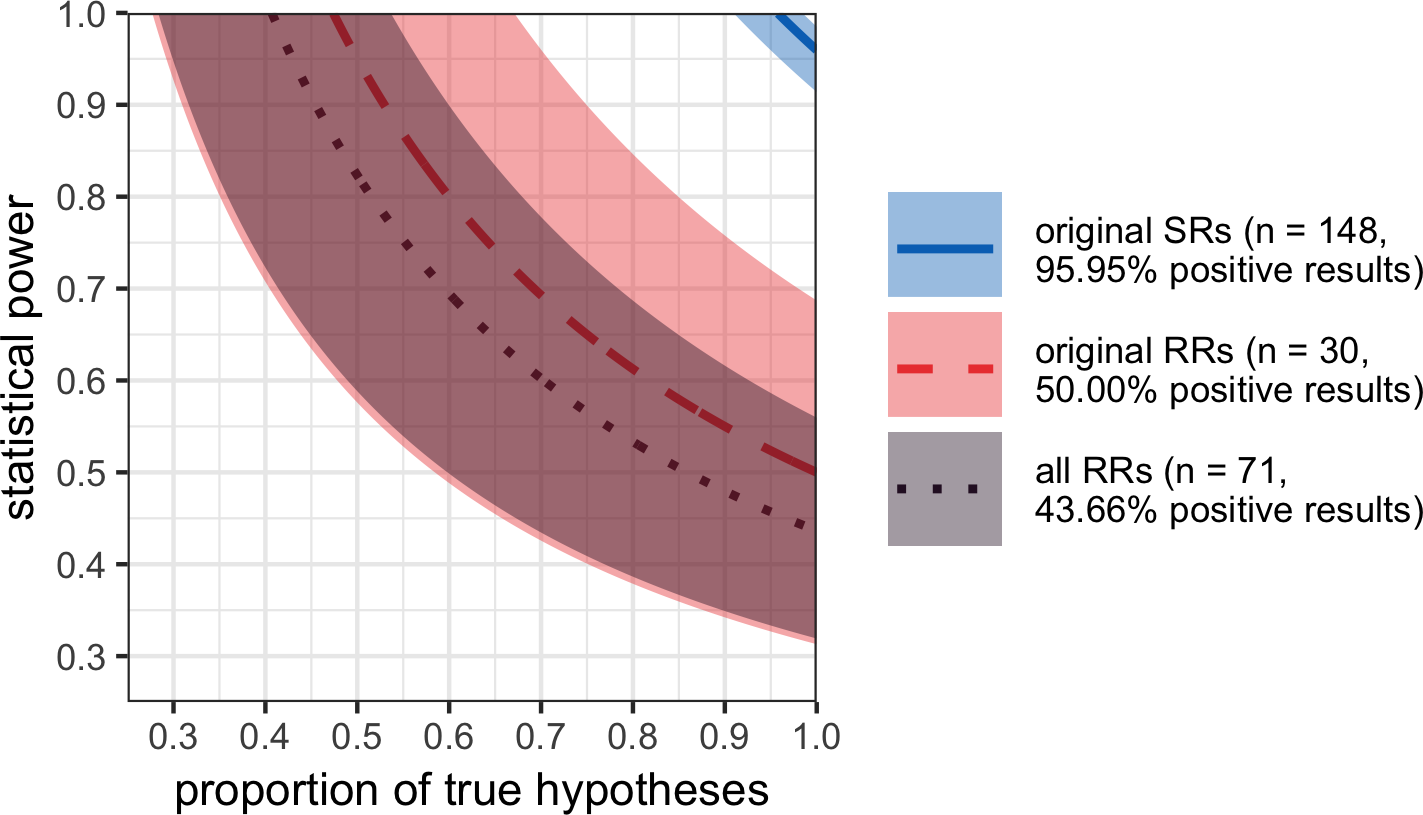
\includegraphics[width=0.6\textwidth]{positive_results_SRs_RRs_files/figure-latex/powerbaserate-1} 

}

\caption{Combinations of the proportion of true hypotheses and statistical power that would produce the observed positive result rates given \(\alpha = 5 \%\) and no bias. Shaded areas indicate \(95\%\) confidence intervals. SRs = standard reports, RRs = Registered Reports. The curve for all SRs (i.e, including replications; \(96.05 \%\) positive results, \(N = 152\)) is not shown because it is almost identical to the one for original SRs. Plotted values were calculated using the equation \(PRR = \alpha*(1-t) + (1-\beta)*t\); with \(PRR =\) positive result rate, \(\alpha =\) probability of obtaining a positive result when testing a false hypothesis (here fixed at .05), \(1-\beta =\) probability of obtaining a positive result when testing a true hypothesis (power), and \(t =\) proportion of true hypotheses; and solving for \(t\) and \(1-\beta\), respectively (with the simplifying assumption that all studies in one group have the same power).}\label{fig:powerbaserate}
\end{figure*}

It is \emph{a-priori} plausible that Registered Reports are currently used for a population of hypotheses that are less likely to be true:
For example, authors may use the format strategically for studies they expect to yield negative results (which would be difficult to publish otherwise).
However, assuming over \(90\%\) true hypotheses in the standard literature is neither realistic, nor would it be desirable for a science that wants to advance knowledge beyond trivial facts.
We thus believe that this factor alone is not sufficient to explain the gap between the positive result rates in Registered Reports and standard reports.
Rather, the numbers strongly suggest a reduction of publication bias and/or Type-1 error inflation in the Registered Reports literature.

\hypertarget{limitations}{%
\subsection{Limitations}\label{limitations}}

We compared hypotheses tested in Registered Reports with hypotheses tested in standard reports.
Because hypotheses, authors, and editors were not randomly assigned to each publication format, we cannot draw firm conclusions about the causes that led to a difference in the proportion of supported hypotheses.
Although it seems plausible that selective reporting and QRPs are reduced in Registered Reports, we do not know by how much, nor if this reduction would be of comparable size in a randomised experiment.
As mentioned above, it is \emph{a-priori} plausible that the Registered Reports format is used selectively for particularly risky hypotheses.
This means that the proportion of true hypotheses in Registered Reports does not necessarily generalise to the entire population of hypotheses that are tested in Psychology.
It is also important to note that our results do not warrant the conclusion that Registered Reports are effective at reducing all forms of bias.
Authors self-select to submit Registered Reports, and the format may be particularly popular among those who try to minimise the risk of inflated error rates regardless of the report format they use.
This would lead to less bias in the Registered Reports literature even if the format's safeguards against certain QRPs were actually ineffective.

A second limitation of the current study (and of Fanelli, 2010) is that standard reports were selected using the search term \enquote{test\(^\ast\) the hypothes\(^\ast\)}.
As our results show, this phrase was virtually absent in the Registered Report population.
The wide variety of ways to introduce a hypothesis we observed in Registered Reports suggests that a search for \enquote{test\(^\ast\) the hypothes\(^\ast\)} might miss most of the hypothesis-testing studies in the psychological literature, and results obtained this way may not generalise to all published studies.
For example, it is possible that authors are more likely to describe their research explicitly as a hypothesis test when they found positive results, but prefer more vague language for unsupported hypotheses (e.g., \enquote{we examined the role of \ldots{}}).
If this were true, using other strategies to select standard reports might yield lower estimates for the positive result rate.
However, this does not seem to be the case:
Studies using different selection criteria for articles and hypotheses have found very similar rates of supported hypotheses.
For example, the positive result rates in Sterling (1959), Sterling et al. (1995), and the original studies included in the Reproducibility Project: Psychology (Open Science Collaboration, 2015) were \(97.28\%\), \(95.56\%\), and \(97\%\), respectively.
Motyl et al. (2017) report \(89.17\%\) and \(92.01\%\) significant results for \enquote{critical} hypothesis tests in papers published in 2003-2004 and 2013-2014, respectively.
Therefore, although the search term used to find standard reports might limit the generalisability of our results, it seems to yield comparable estimates as the selection strategies used in different studies.

A final limitation is the decision to code only the first reported hypothesis.
The first hypothesis test may not be representative for all hypothesis tests reported in a paper, and the order of reporting may differ between standard reports and Registered Reports.
Perhaps Registered-Report authors are more likely to present their hypotheses in \enquote{chronological} order, whereas standard-report authors tend to rearrange the order in which hypotheses are reported based on their outcomes, and present supported hypotheses first.
Here again, the converging estimates from the four studies cited above (none of which use the first-hypothesis rule) make it seem unlikely that our result is an artefact of this decision.
Regardless of which hypothesis one chooses to analyse across a set of papers -- the first, the last, or the \enquote{critical} one -- the positive result rate turns out to be higher than what can be expected based on realistic estimates of the proportion of true hypotheses researchers study and the statistical power of their tests.

\hypertarget{conclusion}{%
\subsection{Conclusion}\label{conclusion}}

Our study presents a systematic comparison of positive results in Registered Reports and the standard literature. The much lower positive result rate in Registered Reports compared to standard reports suggests that an unbiased literature would look very different from the existing body of published research. Standard publication formats seem to lead psychological scientists to miss out on many negative results from high-quality studies, which are available in the Registered Reports literature. The absence of negative results is a serious threat to a cumulative science. In 1959, Sterling asked: \enquote{What credence can then be given to inferences drawn from statistical tests of \(H_0\) if the reader is not aware of all experimental outcomes of a kind?} The amount of experimental outcomes missing from the standard literature appears to be so large that not much credence may be left. In contrast, Registered Reports have clearly led to a much larger proportion of negative results appearing in the literature---and may be one solution to achieve a more credible scientific record.

\hypertarget{disclosures}{%
\subsection{Disclosures}\label{disclosures}}

\hypertarget{data-materials-and-online-resources}{%
\subsubsection{Data, materials, and online resources}\label{data-materials-and-online-resources}}

Data and code necessary to reproduce all analyses reported here, as well as the \href{https://osf.io/qw798/}{Appendix}, the \href{https://osf.io/sy927/}{preregistration}, and additional supplementary files, are available at \url{https://osf.io/dbhgr}. The manuscript including figures and statistical analyses, the \href{https://osf.io/qw798/}{Appendix}, and the \href{https://osf.io/6jrkz/}{codebook} available in the supplement were created using RStudio (1.2.5019, RStudio Team, 2019) and R (Version 3.6.0; R Core Team, 2019) and the R-packages \emph{bookdown} (Version 0.17; Xie, 2016), \emph{codebook} (Version 0.8.2; Arslan, 2018), \emph{ggplot2} (Version 3.1.1; Wickham, 2016), \emph{here} (Version 0.1; Müller, 2017), \emph{knitr} (Version 1.26; Xie, 2015), \emph{papaja} (Version 0.1.0.9842; Aust \& Barth, 2018), \emph{reshape2} (Version 1.4.3; Wickham, 2007), \emph{rio} (Version 0.5.16; Chan, Chan, Leeper, \& Becker, 2018), \emph{rmarkdown} (Version 1.18; Xie, Allaire, \& Grolemund, 2018), \emph{stringr} (Version 1.4.0; Wickham, 2019), and \emph{TOSTER} (Version 0.3.4; Lakens, 2017).

\hypertarget{conflicts-of-interest}{%
\subsubsection{Conflicts of Interest}\label{conflicts-of-interest}}

The authors declare that they have no conflicts of interest with respect to the authorship or the publication of this article.

\hypertarget{author-contributions}{%
\subsubsection{Author Contributions}\label{author-contributions}}

Conceptualisation: A.S. \& D.L.; data curation, formal analysis, and software: A.S. \& M.S.; investigation, methodology, and validation: A.S., M.S., \& D.L; supervision: A.S \& D.L.; visualisation and writing---original draft: A.S; writing---review and editing: A.S., M.S., \& D.L.

\hypertarget{acknowledgements}{%
\subsubsection{Acknowledgements}\label{acknowledgements}}

This work was funded by VIDI grant 452-17-013. We thank Chris Chambers, Emma Henderson, Leonid Tiokhin, and Stuart Ritchie for valuable comments that helped improve this manuscript.

\hypertarget{references}{%
\section{References}\label{references}}

\setlength{\parindent}{-0.2in}
\setlength{\leftskip}{0.2in}

\hypertarget{refs}{}
\leavevmode\hypertarget{ref-Agnoli2017}{}%
Agnoli, F., Wicherts, J. M., Veldkamp, C. L. S., Albiero, P., \& Cubelli, R. (2017). Questionable research practices among italian research psychologists. \emph{PLOS ONE}, \emph{12}(3), e0172792. \url{https://doi.org/10.1371/journal.pone.0172792}

\leavevmode\hypertarget{ref-Allen2019}{}%
Allen, C., \& Mehler, D. M. A. (2019). Open science challenges, benefits and tips in early career and beyond. \emph{PLOS Biology}, \emph{17}(5), e3000246. \url{https://doi.org/10.1371/journal.pbio.3000246}

\leavevmode\hypertarget{ref-R-codebook}{}%
Arslan, R. C. (2018). How to automatically generate rich codebooks from study metadata. PsyArxiv. \url{https://doi.org/10.31234/osf.io/5qc6h}

\leavevmode\hypertarget{ref-Atkinson1982}{}%
Atkinson, D. R., Furlong, M. J., \& Wampold, B. E. (1982). Statistical significance, reviewer evaluations, and the scientific process: Is there a (statistically) significant relationship? \emph{Journal of Counseling Psychology}, \emph{29}(2), 189--194. \url{https://doi.org/10.1037/0022-0167.29.2.189}

\leavevmode\hypertarget{ref-R-papaja}{}%
Aust, F., \& Barth, M. (2018). \emph{papaja: Create APA manuscripts with R Markdown}. Retrieved from \url{https://github.com/crsh/papaja}

\leavevmode\hypertarget{ref-Chambers2013}{}%
Chambers, C. (2013). Registered reports: A new publishing initiative at Cortex, \emph{49}(3), 609--610. Retrieved from \url{http://orca.cf.ac.uk/45177/1/Chambers_Cortex_2013b_GreenOA.pdf}

\leavevmode\hypertarget{ref-Chambers2015}{}%
Chambers, C., Dienes, Z., McIntosh, R., Rotshtein, P., \& Willmes, K. (2015). Registered Reports: Realigning incentives in scientific publishing. \emph{Cortex}, \emph{66}, 1--2. \url{https://doi.org/10.1016/j.cortex.2015.03.022}

\leavevmode\hypertarget{ref-R-rio}{}%
Chan, C.-h., Chan, G. C., Leeper, T. J., \& Becker, J. (2018). \emph{Rio: A swiss-army knife for data file i/o}.

\leavevmode\hypertarget{ref-Cleophas1999}{}%
Cleophas, R. C., \& Cleophas, T. J. (1999). Is selective reporting of clinical research unethical as well as unscientific? \emph{International Journal of Clinical Pharmacology and Therapeutics}, \emph{37}(1), 1--7.

\leavevmode\hypertarget{ref-Cristea2018}{}%
Cristea, I. A., \& Ioannidis, J. P. A. (2018). P values in display items are ubiquitous and almost invariably significant: A survey of top science journals. \emph{PLOS ONE}, \emph{13}(5), e0197440. \url{https://doi.org/10.1371/journal.pone.0197440}

\leavevmode\hypertarget{ref-deWinter2013}{}%
de Winter, J., \& Happee, R. (2013). Why Selective Publication of Statistically Significant Results Can Be Effective. \emph{PLOS ONE}, \emph{8}(6), e66463. \url{https://doi.org/10.1371/journal.pone.0066463}

\leavevmode\hypertarget{ref-Fanelli2010}{}%
Fanelli, D. (2010). "Positive" results increase down the hierarchy of the sciences. \emph{PLoS ONE}, \emph{5}(4), e10068. \url{https://doi.org/10.1371/journal.pone.0010068}

\leavevmode\hypertarget{ref-Fanelli2012}{}%
Fanelli, D. (2012). Negative results are disappearing from most disciplines and countries. \emph{Scientometrics}, \emph{90}(3), 891--904. \url{https://doi.org/10.1007/s11192-011-0494-7}

\leavevmode\hypertarget{ref-Fiedler2016}{}%
Fiedler, K., \& Schwarz, N. (2016). Questionable Research Practices Revisited. \emph{Social Psychological and Personality Science}, \emph{7}(1), 45--52. \url{https://doi.org/10.1177/1948550615612150}

\leavevmode\hypertarget{ref-Franco2014}{}%
Franco, A., Malhotra, N., \& Simonovits, G. (2014). Publication bias in the social sciences: Unlocking the file drawer. \emph{Science}, \emph{345}(6203), 1502--1505. \url{https://doi.org/10.1126/science.1255484}

\leavevmode\hypertarget{ref-Franco2016}{}%
Franco, A., Malhotra, N., \& Simonovits, G. (2016). Underreporting in Psychology Experiments: Evidence From a Study Registry. \emph{Social Psychological and Personality Science}, \emph{7}(1), 8--12. \url{https://doi.org/10.1177/1948550615598377}

\leavevmode\hypertarget{ref-Goldacre2016}{}%
Goldacre, B., Drysdale, H., Powell-Smith, A., Dale, A., Milosevic, I., Slade, E., \ldots{} Heneghan, C. (2016). The COMPare Trials Project. Retrieved February 3, 2020, from \url{http://compare-trials.org}

\leavevmode\hypertarget{ref-Greenwald1975}{}%
Greenwald, A. G. (1975). Consequences of Prejudice Against the Null Hypothesis. \emph{Psychological Bulletin}, \emph{82}(1), 1--20.

\leavevmode\hypertarget{ref-John2012}{}%
John, L. K., Loewenstein, G., \& Prelec, D. (2012). Measuring the Prevalence of Questionable Research Practices With Incentives for Truth Telling. \emph{Psychological Science}, \emph{23}(5), 524--532. \url{https://doi.org/10.1177/0956797611430953}

\leavevmode\hypertarget{ref-Jonas2016}{}%
Jonas, K. J., \& Cesario, J. (2016). How can preregistration contribute to research in our field? \emph{Comprehensive Results in Social Psychology}, \emph{1}(1-3), 1--7. \url{https://doi.org/10.1080/23743603.2015.1070611}

\leavevmode\hypertarget{ref-Kaplan2015}{}%
Kaplan, R. M., \& Irvin, V. L. (2015). Likelihood of Null Effects of Large NHLBI Clinical Trials Has Increased over Time. \emph{PLOS ONE}, \emph{10}(8), e0132382. \url{https://doi.org/10.1371/journal.pone.0132382}

\leavevmode\hypertarget{ref-Kerr1998}{}%
Kerr, N. L. (1998). HARKing: Hypothesizing after the results are known. \emph{Personality and Social Psychology Review}, \emph{2}(3), 196--217. \url{https://doi.org/10.1207/s15327957pspr0203_4}

\leavevmode\hypertarget{ref-Kohler2019}{}%
Köhler, T., \& Cortina, J. M. (2019). Play It Again, Sam! An Analysis of Constructive Replication in the Organizational Sciences. \emph{Journal of Management}, 014920631984398. \url{https://doi.org/10.1177/0149206319843985}

\leavevmode\hypertarget{ref-R-TOSTER}{}%
Lakens, D. (2017). Equivalence tests: A practical primer for t-tests, correlations, and meta-analyses. \emph{Social Psychological and Personality Science}, \emph{1}, 1--8. \url{https://doi.org/10.1177/1948550617697177}

\leavevmode\hypertarget{ref-Lakens2019b}{}%
Lakens, D. (2019). The Value of Preregistration for Psychological Science: A Conceptual Analysis. \url{https://doi.org/10.31234/osf.io/jbh4w}

\leavevmode\hypertarget{ref-Lakens2018a}{}%
Lakens, D., Scheel, A. M., \& Isager, P. M. (2018). Equivalence Testing for Psychological Research: A Tutorial. \emph{Advances in Methods and Practices in Psychological Science}, \emph{1}(2), 259--269. \url{https://doi.org/10.1016/j.ympev.2015.01.015}

\leavevmode\hypertarget{ref-Mahoney1977}{}%
Mahoney, M. J. (1977). Publication Prejudices: An Experimental Study of Confirmatory Bias in the Peer Review System. \emph{Cognitive Therapy and Research}, \emph{1}(2), 161--175. \url{https://doi.org/10.1007/BF01173636}

\leavevmode\hypertarget{ref-Makel2012}{}%
Makel, M. C., Plucker, J. A., \& Hegarty, B. (2012). Replications in Psychology Research: How Often Do They Really Occur? \emph{Perspectives on Psychological Science}. \url{https://doi.org/10.1177/1745691612460688}

\leavevmode\hypertarget{ref-Maxwell2004}{}%
Maxwell, S. E. (2004). The Persistence of Underpowered Studies in Psychological Research: Causes, Consequences, and Remedies. \emph{Psychological Methods}, \emph{9}(2), 147--163. \url{https://doi.org/10.1037/1082-989X.9.2.147}

\leavevmode\hypertarget{ref-Motyl2017}{}%
Motyl, M., Demos, A. P., Carsel, T. S., Hanson, B. E., Melton, Z. J., Mueller, A. B., \ldots{} Skitka, L. J. (2017). The state of social and personality science: Rotten to the core, not so bad, getting better, or getting worse? \emph{Journal of Personality and Social Psychology}, \emph{113}(1), 34--58. \url{https://doi.org/10.1037/pspa0000084}

\leavevmode\hypertarget{ref-Mueller-Langer2019}{}%
Mueller-Langer, F., Fecher, B., Harhoff, D., \& Wagner, G. G. (2019). Replication studies in economics---How many and which papers are chosen for replication, and why? \emph{Research Policy}, \emph{48}(1), 62--83. \url{https://doi.org/10.1016/j.respol.2018.07.019}

\leavevmode\hypertarget{ref-R-here}{}%
Müller, K. (2017). \emph{Here: A simpler way to find your files}. Retrieved from \url{https://CRAN.R-project.org/package=here}

\leavevmode\hypertarget{ref-Nosek2014}{}%
Nosek, B. A., \& Lakens, D. (2014). Registered Reports: A Method to Increase the Credibility of Published Results. \emph{Social Psychology}, \emph{45}(3), 137--141. \url{https://doi.org/10.1027/1864-9335/a000192}

\leavevmode\hypertarget{ref-OSC2015}{}%
Open Science Collaboration. (2015). Estimating the reproducibility of psychological science. \emph{Science}, \emph{349}(6251), aac4716. \url{https://doi.org/10.1126/science.aac4716}

\leavevmode\hypertarget{ref-Pridemore2018}{}%
Pridemore, W. A., Makel, M. C., \& Plucker, J. A. (2018). Replication in Criminology and the Social Sciences. \emph{Annual Review of Criminology}, \emph{1}(1), 19--38. \url{https://doi.org/10.1146/annurev-criminol-032317-091849}

\leavevmode\hypertarget{ref-Rasmussen2009}{}%
Rasmussen, N., Lee, K., \& Bero, L. (2009). Association of trial registration with the results and conclusions of published trials of new oncology drugs. \emph{Trials}, \emph{10}(1), 116. \url{https://doi.org/10.1186/1745-6215-10-116}

\leavevmode\hypertarget{ref-R-base}{}%
R Core Team. (2019). \emph{R: A language and environment for statistical computing}. Vienna, Austria: R Foundation for Statistical Computing. Retrieved from \url{https://www.R-project.org/}

\leavevmode\hypertarget{ref-RRRwebsite}{}%
Registered Replication Reports. (n.d.). Retrieved December 28, 2019, from \url{https://www.psychologicalscience.org/publications/replication}

\leavevmode\hypertarget{ref-Rohatgi2018}{}%
Rohatgi, A. (2018). \emph{WebPlotDigitizer - Web Based Plot Digitizer}. Austin, Texas, USA. Retrieved from \url{https://automeris.io/WebPlotDigitizer}

\leavevmode\hypertarget{ref-Rosenthal1979}{}%
Rosenthal, R. (1979). The file drawer problem and tolerance for null results. \emph{Psychological Bulletin}, \emph{86}(3), 638--641. \url{https://doi.org/10.1037/0033-2909.86.3.638}

\leavevmode\hypertarget{ref-RStudioTeam2019}{}%
RStudio Team. (2019). \emph{RStudio: Integrated development environment for r}. Boston, MA: RStudio, Inc. Retrieved from \url{http://www.rstudio.com/}

\leavevmode\hypertarget{ref-Simmons2011}{}%
Simmons, J. P., Nelson, L. D., \& Simonsohn, U. (2011). False-positive psychology: Undisclosed flexibility in data collection and analysis allows presenting anything as significant. \emph{Psychological Science}, \emph{22}(11), 1359--1366. \url{https://doi.org/10.1177/0956797611417632}

\leavevmode\hypertarget{ref-Simons2018}{}%
Simons, D. J. (2018). Introducing Advances in Methods and Practices in Psychological Science. \emph{Advances in Methods and Practices in Psychological Science}, \emph{1}(1), 3--6. \url{https://doi.org/10.1177/2515245918757424}

\leavevmode\hypertarget{ref-Simons2014}{}%
Simons, D. J., Holcombe, A. O., \& Spellman, B. A. (2014). An Introduction to Registered Replication Reports at \emph{Perspectives} \emph{on} \emph{Psychological Science}. \emph{Perspectives on Psychological Science}, \emph{9}(5), 552--555. \url{https://doi.org/10.1177/1745691614543974}

\leavevmode\hypertarget{ref-SingletonThorn2019}{}%
Singleton Thorn, F., Dudgeon, P., \& Fidler, F. (2019, September). \emph{Statistical power and effect sizes in psychology are decreasing over time}. Presented at the Metascience 2019 Symposium, Stanford, CA, USA. Retrieved from \url{https://www.metascience2019.org/poster-session/felix-singleton-thorn/}

\leavevmode\hypertarget{ref-Sterling1959}{}%
Sterling, T. D. (1959). Publication Decisions and their Possible Effects on Inferences Drawn from Tests of Significance---or Vice Versa. \emph{Journal of the American Statistical Association}, \emph{54}(285), 30--34. \url{https://doi.org/10.1080/01621459.1959.10501497}

\leavevmode\hypertarget{ref-Sterling1995}{}%
Sterling, T. D., Rosenbaum, W. L., \& Weinkam, J. J. (1995). Publication Decisions Revisited: The Effect of the Outcome of Statistical Tests on the Decision to Publish and Vice Versa. \emph{The American Statistician}, \emph{49}(1), 108. \url{https://doi.org/10.2307/2684823}

\leavevmode\hypertarget{ref-Szucs2017}{}%
Szucs, D., \& Ioannidis, J. P. A. (2017). Empirical assessment of published effect sizes and power in the recent cognitive neuroscience and psychology literature. \emph{PLOS Biology}, \emph{15}(3), e2000797. \url{https://doi.org/10.1371/journal.pbio.2000797}

\leavevmode\hypertarget{ref-vanAssen2014}{}%
van Assen, M. A. L. M., van Aert, R. C. M., Nuijten, M. B., \& Wicherts, J. M. (2014). Why Publishing Everything Is More Effective than Selective Publishing of Statistically Significant Results. \emph{PLOS ONE}, \emph{9}(1), e84896. \url{https://doi.org/10.1371/journal.pone.0084896}

\leavevmode\hypertarget{ref-R-reshape2}{}%
Wickham, H. (2007). Reshaping data with the reshape package. \emph{Journal of Statistical Software}, \emph{21}(12), 1--20. Retrieved from \url{http://www.jstatsoft.org/v21/i12/}

\leavevmode\hypertarget{ref-R-ggplot2}{}%
Wickham, H. (2016). \emph{Ggplot2: Elegant graphics for data analysis}. Springer-Verlag New York. Retrieved from \url{https://ggplot2.tidyverse.org}

\leavevmode\hypertarget{ref-R-stringr}{}%
Wickham, H. (2019). \emph{Stringr: Simple, consistent wrappers for common string operations}. Retrieved from \url{https://CRAN.R-project.org/package=stringr}

\leavevmode\hypertarget{ref-Wiseman2019}{}%
Wiseman, R., Watt, C., \& Kornbrot, D. (2019). Registered reports: An early example and analysis. \emph{PeerJ}, \emph{7}, e6232. \url{https://doi.org/10.7717/peerj.6232}

\leavevmode\hypertarget{ref-R-knitr}{}%
Xie, Y. (2015). \emph{Dynamic documents with R and knitr} (2nd ed.). Boca Raton, Florida: Chapman; Hall/CRC. Retrieved from \url{https://yihui.name/knitr/}

\leavevmode\hypertarget{ref-R-bookdown}{}%
Xie, Y. (2016). \emph{Bookdown: Authoring books and technical documents with R markdown}. Boca Raton, Florida: Chapman; Hall/CRC. Retrieved from \url{https://github.com/rstudio/bookdown}

\leavevmode\hypertarget{ref-R-rmarkdown}{}%
Xie, Y., Allaire, J., \& Grolemund, G. (2018). \emph{R markdown: The definitive guide}. Boca Raton, Florida: Chapman; Hall/CRC. Retrieved from \url{https://bookdown.org/yihui/rmarkdown}

\end{document}
